\PassOptionsToPackage{unicode=true}{hyperref} % options for packages loaded elsewhere
\PassOptionsToPackage{hyphens}{url}
%
\documentclass[ignorenonframetext,]{beamer}
\usepackage{pgfpages}
\setbeamertemplate{caption}[numbered]
\setbeamertemplate{caption label separator}{: }
\setbeamercolor{caption name}{fg=normal text.fg}
\beamertemplatenavigationsymbolsempty
\usepackage{lmodern}
\usepackage{amssymb,amsmath}
\usepackage{ifxetex,ifluatex}
\usepackage{fixltx2e} % provides \textsubscript
\ifnum 0\ifxetex 1\fi\ifluatex 1\fi=0 % if pdftex
  \usepackage[T1]{fontenc}
  \usepackage[utf8]{inputenc}
  \usepackage{textcomp} % provides euro and other symbols
\else % if luatex or xelatex
  \usepackage{unicode-math}
  \defaultfontfeatures{Ligatures=TeX,Scale=MatchLowercase}
\fi
% use upquote if available, for straight quotes in verbatim environments
\IfFileExists{upquote.sty}{\usepackage{upquote}}{}
% use microtype if available
\IfFileExists{microtype.sty}{%
\usepackage[]{microtype}
\UseMicrotypeSet[protrusion]{basicmath} % disable protrusion for tt fonts
}{}
\IfFileExists{parskip.sty}{%
\usepackage{parskip}
}{% else
\setlength{\parindent}{0pt}
\setlength{\parskip}{6pt plus 2pt minus 1pt}
}
\usepackage{hyperref}
\hypersetup{
            pdftitle={Introduction},
            pdfauthor={Mbah Boedy},
            pdfborder={0 0 0},
            breaklinks=true}
\urlstyle{same}  % don't use monospace font for urls
\newif\ifbibliography
\usepackage{graphicx,grffile}
\makeatletter
\def\maxwidth{\ifdim\Gin@nat@width>\linewidth\linewidth\else\Gin@nat@width\fi}
\def\maxheight{\ifdim\Gin@nat@height>\textheight\textheight\else\Gin@nat@height\fi}
\makeatother
% Scale images if necessary, so that they will not overflow the page
% margins by default, and it is still possible to overwrite the defaults
% using explicit options in \includegraphics[width, height, ...]{}
\setkeys{Gin}{width=\maxwidth,height=\maxheight,keepaspectratio}
% Prevent slide breaks in the middle of a paragraph:
\widowpenalties 1 10000
\raggedbottom
\setbeamertemplate{part page}{
\centering
\begin{beamercolorbox}[sep=16pt,center]{part title}
  \usebeamerfont{part title}\insertpart\par
\end{beamercolorbox}
}
\setbeamertemplate{section page}{
\centering
\begin{beamercolorbox}[sep=12pt,center]{part title}
  \usebeamerfont{section title}\insertsection\par
\end{beamercolorbox}
}
\setbeamertemplate{subsection page}{
\centering
\begin{beamercolorbox}[sep=8pt,center]{part title}
  \usebeamerfont{subsection title}\insertsubsection\par
\end{beamercolorbox}
}
\AtBeginPart{
  \frame{\partpage}
}
\AtBeginSection{
  \ifbibliography
  \else
    \frame{\sectionpage}
  \fi
}
\AtBeginSubsection{
  \frame{\subsectionpage}
}
\setlength{\emergencystretch}{3em}  % prevent overfull lines
\providecommand{\tightlist}{%
  \setlength{\itemsep}{0pt}\setlength{\parskip}{0pt}}
\setcounter{secnumdepth}{0}

% set default figure placement to htbp
\makeatletter
\def\fps@figure{htbp}
\makeatother


\title{Introduction}
\author{Mbah Boedy}
\date{}

\begin{document}
\frame{\titlepage}

\begin{frame}{Welcome}
\protect\hypertarget{welcome}{}

Welcome to Algorithms class :)

\end{frame}

\begin{frame}{Lecturer}
\protect\hypertarget{lecturer}{}

\begin{itemize}
\tightlist
\item
  This class will be delivered by
  \href{http://it.maranatha.edu/resume/setiabudi/}{Setia Budi}
\item
  Feel free to call me Mbah Boedy :)
\item
  Consultation time is provided for the students to discuss any matter
  realated to the class
\item
  Consultation time: Friday from 12:30 to 1:30 pm at GWM lv.8
\item
  Email:
  \href{mailto:Setia.Budi@it.maranatha.edu}{\nolinkurl{Setia.Budi@it.maranatha.edu}}
\end{itemize}

\end{frame}

\begin{frame}{Textbook}
\protect\hypertarget{textbook}{}

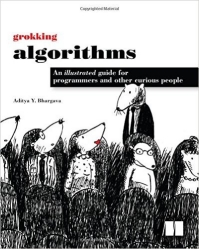
\includegraphics{./Introduction-figure/textbook.jpg}

\begin{itemize}
\tightlist
\item
  The lecture in this class will be delivered based on a textbook
\item
  Title:
  \href{https://www.manning.com/books/grokking-algorithms}{Grokking
  Algorithms}
\item
  Authors: Aditya Y. Bhargava\\
\item
  Publisher: Manning, 2016
\end{itemize}

\end{frame}

\begin{frame}{Softwares}
\protect\hypertarget{softwares}{}

\begin{itemize}
\tightlist
\item
  Operating Systems: Windows / MacOS / Linux
\item
  Text Editor: \href{https://code.visualstudio.com/}{Visual Studio Code}
\item
  Python 3 distribution:
  \href{https://www.anaconda.com/download/}{Anaconda}
\item
  Web Browser:
  \href{https://www.mozilla.org/en-US/firefox/new/}{Firefox} or
  \href{https://www.google.com/chrome/browser/desktop/index.html}{Chrome}
\end{itemize}

\end{frame}

\begin{frame}{Grading}
\protect\hypertarget{grading}{}

\begin{itemize}
\tightlist
\item
  KAT {[}50\%{]}:

  \begin{itemize}
  \tightlist
  \item
    Attendance (15\%)
  \item
    Engagement (15\%)
  \item
    Online Quiz (20\%)
  \end{itemize}
\item
  UTS {[}25\%{]}: Written Exam
\item
  UAS {[}25\%{]}: Written Exam
\end{itemize}

\end{frame}

\begin{frame}{Engagement Slip}
\protect\hypertarget{engagement-slip}{}

\begin{itemize}
\tightlist
\item
  Each engagement in the class is entitled for an engagement mark.
\item
  Please fill your student id and name on the engagement sheet as a
  record of your engagement.
\item
  Maximum one engagement mark per week.
\end{itemize}

\end{frame}

\begin{frame}{Google Classroom}
\protect\hypertarget{google-classroom}{}

\begin{itemize}
\tightlist
\item
  We are going to use Google Classroom as Learning Management System
\item
  Get access to lecture slides and other learning resources
\item
  Get access to weekly quizes
\item
  Get access to weekly marks
\item
  Please download and install it to your Android device via
  \href{https://play.google.com/store/apps/details?id=com.google.android.apps.classroom}{Playstore}
\item
  You can also get access via a web browser:
  \url{https://classroom.google.com/}
\end{itemize}


\includegraphics{./Introduction-figure/Google-Classroom-Logo.png}

\end{frame}

\begin{frame}{Introducing IBAtS}
\protect\hypertarget{introducing-ibats}{}

\begin{itemize}
\tightlist
\item
  IBAtS is an Image Based Attendance System to record students
  attendance in a class.
\item
  We are going to use IBAtS in this class (on top of the conventional
  attendance system).
\item
  Please download it to your Android device via
  \href{https://play.google.com/store/apps/details?id=iBatsForStudent.Android}{PlayStore}.
\end{itemize}


\includegraphics{./Introduction-figure/ibats.png}

\end{frame}

\begin{frame}{General Rules}
\protect\hypertarget{general-rules}{}

\begin{itemize}
\tightlist
\item
  Be punctual, the lecture will start on time.
\item
  Be respectful to others, no bullying in this class.
\item
  Don't be hasitate to ask question if you have any difficulty in the
  class.
\item
  Asking question and discussion are part of learning process.
\item
  Being confused in the begining is a good indication that you are
  actually` learning something new, but don't leave it too long.
\item
  Please study the textbook before and after the class.
\item
  A study group could be a good way to learn from each other.
\item
  Enjoy the class :)
\end{itemize}

\end{frame}

\end{document}
